\documentclass[a4paper,14pt]{extarticle}

\usepackage[utf8x]{inputenc}
\usepackage[T1,T2A]{fontenc}
\usepackage[russian]{babel}
\usepackage{hyperref}
\usepackage{indentfirst}
\usepackage{here}
\usepackage{array}
\usepackage{graphicx}
\usepackage{caption}
\usepackage{subcaption}
\usepackage{chngcntr}
\usepackage{amsmath}
\usepackage{amssymb}
\usepackage{pgfplots}
\usepackage{pgfplotstable}
\usepackage[left=2cm,right=2cm,top=2cm,bottom=2cm,bindingoffset=0cm]{geometry}
\usepackage{multicol}
\usepackage{askmaps}
\usepackage{titlesec}
\usepackage{listings}
\usepackage{color}
\usepackage{courier}

\definecolor{green}{rgb}{0,0.6,0}
\definecolor{gray}{rgb}{0.5,0.5,0.5}
\definecolor{purple}{rgb}{0.58,0,0.82}

\lstset{
	language=Verilog,
	backgroundcolor=\color{white},   
	basicstyle=\small\ttfamily,
	commentstyle=\color{green},
	keywordstyle=\color{blue},	
	numberstyle=\tiny\color{gray},
	stringstyle=\color{purple},
	breakatwhitespace=false,
	breaklines=true,
	captionpos=b,
	keepspaces=true,
	numbers=left,
	numbersep=5pt,
	showspaces=false,
	showstringspaces=false,
	showtabs=false,
	tabsize=4,
	frame=single,
	inputpath={../quartus/},
	literate={~} {$\sim$}{1}
}

\renewcommand{\le}{\ensuremath{\leqslant}}
\renewcommand{\leq}{\ensuremath{\leqslant}}
\renewcommand{\ge}{\ensuremath{\geqslant}}
\renewcommand{\geq}{\ensuremath{\geqslant}}
\renewcommand{\epsilon}{\ensuremath{\varepsilon}}
\renewcommand{\phi}{\ensuremath{\varphi}}
\renewcommand{\thefigure}{\arabic{figure}} 	
\renewcommand*\not[1]{\overline{#1}}

\titleformat*{\section}{\large\bfseries} 
\titleformat*{\subsection}{\normalsize\bfseries} 
\titleformat*{\subsubsection}{\normalsize\bfseries} 
\titleformat*{\paragraph}{\normalsize\bfseries} 
\titleformat*{\subparagraph}{\normalsize\bfseries} 

\counterwithin{figure}{section}
\counterwithin{equation}{section}
\counterwithin{table}{section}
\newcommand{\sign}[1][5cm]{\makebox[#1]{\hrulefill}}
\graphicspath{{../pics/}}
\captionsetup{justification=centering,margin=1cm}
\def\arraystretch{1.3}
\setlength\parindent{5ex}
\titlelabel{\thetitle.\quad}

\begin{document}

\begin{titlepage}
\begin{center}
	Санкт-Петербургский Политехнический Университет Петра Великого\\[0.3cm]
	Институт компьютерных наук и технологий \\[0.3cm]
	Кафедра компьютерных систем и программных технологий\\[4cm]
	
	\textbf{ОТЧЕТ}\\ 
	\textbf{по лабораторной работе}\\[0.5cm]
	\textbf{SystemVerilog №4}\\[0.1cm]
	Автоматизация проектирования\\ дискретных устройств\\[4.0cm]
\end{center}

\begin{flushright}
	\begin{minipage}{0.45\textwidth}
		\textbf{Работу выполнил студент}\\[3mm]
		группа 33501/4 \hspace*{9mm} Дьячков В.В.\\[5mm]
		\textbf{Преподаватель}\\[5mm]
		\sign[1.5cm] \hspace*{1mm} к.т.н., доц. Филиппов А.С. \\[5mm]
	\end{minipage}
\end{flushright}

\vfill

\begin{center}
	Санкт-Петербург\\
	\the\year
\end{center}
\end{titlepage}

\addtocounter{page}{1}
\counterwithin{lstlisting}{section}

\tableofcontents
\listoffigures
\lstlistoflistings
\newpage

\section{Задачи работы}

\begin{enumerate}
\setlength\itemsep{0em}
\item Задание требований к тактовой частоте проекта.
\item Работа с приложением TimeQuest.
\item Анализ полученных результатов для максимальной тактовой частоты работы устройства.
\end{enumerate}

\section{Синтез 4-разрядного счетчика}

\subsection{Результаты синтеза}

На рис. \ref{fig:counter} изображена синтезированная схема 4-разрядного счетчика.

\begin{figure}[H]
\begin{center}
	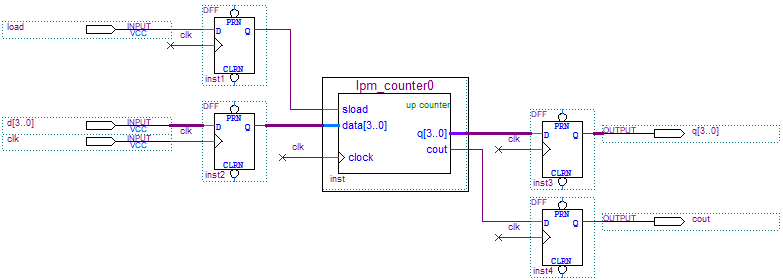
\includegraphics[width=\textwidth]{counter}
	\caption{Синтезированная схема}
	\label{fig:counter}
\end{center}
\end{figure}

\vspace{-0.5cm}
\subsection{Результаты моделирования}

На рис. \ref{fig:func-modeling} изображен результат функционального моделирования, полученный с помощью встроенной системы моделирования – University Program VWF.

\vspace{-0.5cm}
\begin{figure}[H]
\begin{center}
	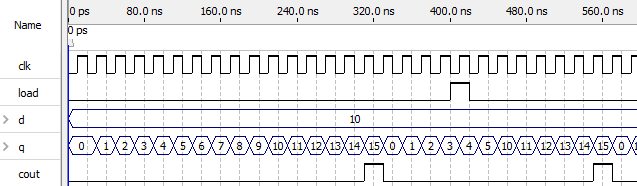
\includegraphics[scale=0.9]{modeling}
	\caption{Результаты моделирования}
	\label{fig:func-modeling}
\end{center}
\end{figure}

%TODO Проведите анализ временной диаграммы и объясните почему:
%TODO Данные записываемые в счетчик появляются на выходе с задержкой 2 такта?
%TODO В самом начале моделирования значение 0 присутствует на выходе 2 такта?

\subsection{Временной анализ}

\subsubsection{Создание SDC файла}

В листинге \ref{code:sdc} приведена сформированная SDC команда, создающая ограничения для тактового сигнала.

\begin{lstlisting}[caption=Synopsys Design Constraints (SDC) файл, label=code:sdc]
create_clock -name input_clk -period 20.000 [get_ports {clk}]
\end{lstlisting}

В отчете компиляции в разделе \textbf{TimeQuest Timing Analyzer} указана максимальная тактовая частота работы проекта: Fmax = $465.55$ MHz, Restricted Fmax = $250$ MHz.

В таблице \textbf{Multicorner Timing Analysis Summary} приведены следующие значения задержек для худшего случая:
\begin{itemize}
\setlength\itemsep{0em}
\item Setup Slack = $17.852$ нс.
\item Hold Slack = $0.197$ нс.
\item Slack для Minimum Pulse Width = $9.436$ нс.
\end{itemize}

\subsubsection{Изменение периода тактового сигнала}

При изменении ограничения с 20 нс до 1 нс (то есть частота работы $10$0 MHz), максимальная тактовая частота стала следующей: Fmax = $489.24$ MHz, Restricted Fmax = $250$ MHz. Из результатов видно, что значение Fmax увеличилось.

В таблице \textbf{Multicorner Timing Analysis Summary} значения задержек стали равны:
\begin{itemize}
\setlength\itemsep{0em}
\item Setup Slack = $-1.044$ нс.
\item Hold Slack = $0.256$ нс.
\item Slack для Minimum Pulse Width = $-3.000$ нс.
\end{itemize}
%TODO Объясните с какими параметрами возникли проблемы

\subsubsection{Анализ временных диаграмм}

На рис. \ref{fig:waveform_setup} и \ref{fig:waveform_hold} изображены временные диаграммы распространения данных и тактового сигнала для анализа Setup Slask и Hold Slack соответственно.

\begin{figure}[H]
\begin{center}
	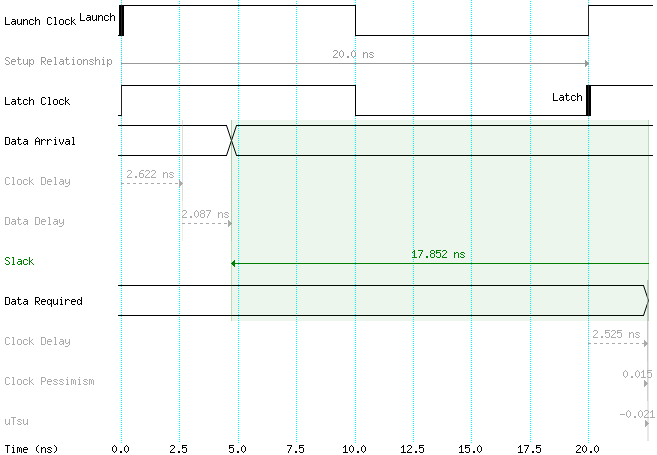
\includegraphics[scale=0.9]{waveform_setup}
	\caption{Временная диаграмма Setup анализа}
	\label{fig:waveform_setup}
\end{center}
\end{figure}
%TODO Найдите на ней параметры, использованные в лекции для анализа зазора Setup Slack.
\vspace{-1.5cm}
\begin{figure}[H]
\begin{center}
	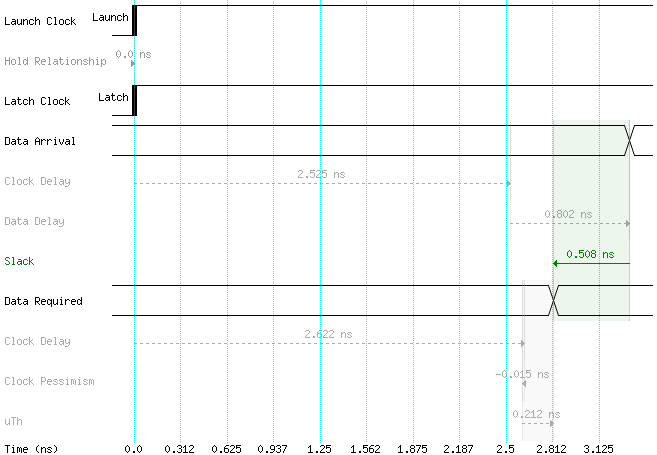
\includegraphics[scale=0.9]{waveform_hold}
	\caption{Временная диаграмма Hold анализа}
	\label{fig:waveform_hold}
\end{center}
\end{figure}
%TODO Найдите на ней параметры, использованные в лекции для анализа зазоров Slack Hold

\section{Синтез 128-разрядного счетчика}

\subsection{Временной анализ}

\subsubsection{Максимальная частота}

В отчете компиляции в разделе \textbf{TimeQuest Timing Analyzer} указана максимальная тактовая частота работы проекта: Fmax = $180.21$ MHz, Restricted Fmax = $180.21$ MHz. Следовательно требование к максимальной тактовой частоте выполнено.  
%TODO Какая максимально допустимая тактовая частота работы проекта?

\subsubsection{Критический путь}

Setup Slack для критического пути (пути для которого максимальный отрицательный Slack) оказался равен $-1.549$ нс.
%TODO Сколько критических путей – путей ограничивающих тактовую частоту? 2?

\begin{figure}[H]
\begin{center}
	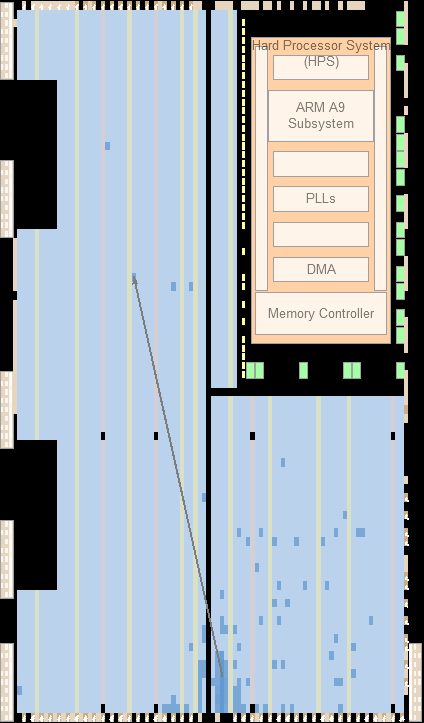
\includegraphics[scale=0.75]{chip_planner}
	\caption{Путь между двумя триггерами, определяющими критический путь, в редакторе Chip Planner}
	\label{fig:chip_planner}
\end{center}
\end{figure}

\section{Выводы}

\end{document}